\documentclass[a4paper,10pt]{report}

\topmargin -2cm
%\topskip0cm
%\footskip0cm
%\headsep0cm
\parindent0cm
\oddsidemargin -1cm
\evensidemargin -1cm
\headheight 2cm
\textheight 24cm
\textwidth 18cm

\author{Daniel W\"aber (4049590)}
\title{\"Ubung}

\usepackage{ucs}
\usepackage[utf8x]{inputenc}
\usepackage{german}
\usepackage{color}
\usepackage{url}
\usepackage{graphicx}
\usepackage{algorithmic}

\pagestyle{empty}
\usepackage{makeidx}
\usepackage{amsmath}
\usepackage{amsfonts}
\usepackage{amssymb,euscript}
\usepackage{dsfont}
\usepackage{listings}
\usepackage{enumerate}
\newfont{\Fr}{eufm10}
\newfont{\Sc}{eusm10}
\newfont{\Bb}{msbm10}
\newcommand{\limin}{\lim_{n\rightarrow\infty}}
\newcommand{\limix}{\lim_{x\rightarrow\infty}}
\newcommand{\limun}{\lim_{n\rightarrow -\infty}}
\newcommand{\limux}{\lim_{n\rightarrow -\infty}}
\newcommand{\limx}{\lim_{x\rightarrow x_0}}
\newcommand{\limh}{\lim_{h\rightarrow 0}}
\newcommand{\defi}{\paragraph{Definition:}}
\newcommand{\bew}{\paragraph{Beweis:}}
\newcommand{\satz}{\paragraph{Satz:}}
\newcommand{\bsp}{\paragraph{Beispiel:}}
\newcommand{\lemma}{\paragraph{Lemma:}}
\newcommand{\N}{\mathds{N}}
\newcommand{\F}{\mathds{F}}
\newcommand{\Z}{\mathds{Z}}
\newcommand{\Q}{\mathds{Q}}
\newcommand{\R}{\mathds{R}}
\newcommand{\G}{\mathds{G}}
\newcommand{\C}{\mathds{C}}
\newcommand{\K}{\mathds{K}}
\newcommand{\A}{\mathds{A}}
\newcommand{\E}{\mathcal{E}}
\renewcommand{\P}{\mathcal{P}}
\newcommand{\sigA}{$\sigma$-Algebra }
\newcommand{\qed}{$\hfill\blacksquare$}
\newcommand{\arsinh}{\operatorname{arsinh} }
\newcommand{\arcosh}{\operatorname{arcosh} }
\newcommand{\gdw}{ $ \Leftrightarrow $ }
\newcommand{\tf}{ $ \Rightarrow $ }
\newcommand{\mgdw}{\Leftrightarrow}
\newcommand{\mtf}{\Rightarrow}
\newcommand{\Bild}{\text{Bild}}
\newcommand{\Kern}{\text{kern}}
\newcommand{\rg}{\text{rg}}
\newcommand{\deff}{\text{deff}}

\newcommand{\alphato}{\underset{\alpha}\to}
\newcommand{\betato}{\underset{\beta}\to}
\newcommand{\etato}{\underset{\eta}\to}
\newcommand{\ito}{\underset{i}\to}
\newcommand{\sto}{\underset{s}\to}
\newcommand{\kto}{\underset{k}\to}
\newcommand{\xto}{\underset{x}\to}

\usepackage{fancyhdr}
\pagestyle{fancy}
\lhead{Daniel Waeber\\Alex Muenn}
\chead{"Ubungsblatt \nr\\\today}
\rhead{Bildverarbeitung}


\newcommand{\nr}{5}
\lstset{language=matlab}

\begin{document}
\section*{Aufgabe 1 - Lifting CDF(2,2)}
Die des CDF(2,2)-Liftingverfahrens ist in einer 1:1 Umsetzung m\"oglich,
wenn man ber\"ucksichtigt, dass an den R\"andern fur $d_{j-1}[1]$ kein
$S_{j}[0]$ existiert und dieses durch zB mit $0$ besetzt werden muss.
\\
In der Durchf\"uhrung werden die Bildpunkte nach gerade und ungerade 
aufgeteilt. Zur Prediction wird nun zu jedem Wert der geraden Bildpunkt 
der Vorg\"anger addiert, was sich sehr gut als Vektoroperation schreiben
l\"asst:
\\
\begin{eqnarray}
\vec{P} &=&  \vec{S}_{j}[2:2:n] + \left(\begin{array}{c}0\\\vec{S}_{j}[2:2:n-1]\end{array}\right)\\
\vec{D}_{j-1} &=&  \vec{S}_{j-1}[1:2:n] - \frac{1}{2} \cdot \vec{P}\\
\vec{S}_{j-1} &=&  \vec{S}_{j}[2:2:n] + \frac{1}{4} \cdot (\vec{D}_{j-1} + \vec{D}_{j-1}^{zeroshift})
\end{eqnarray}

$\vec{S}_{j-1}$ fliesst solange in CDF(2,2) ein bis nur noch ein (ungerades Element)
\"ubrig bleibt.


\begin{figure}[H]
\begin{center}
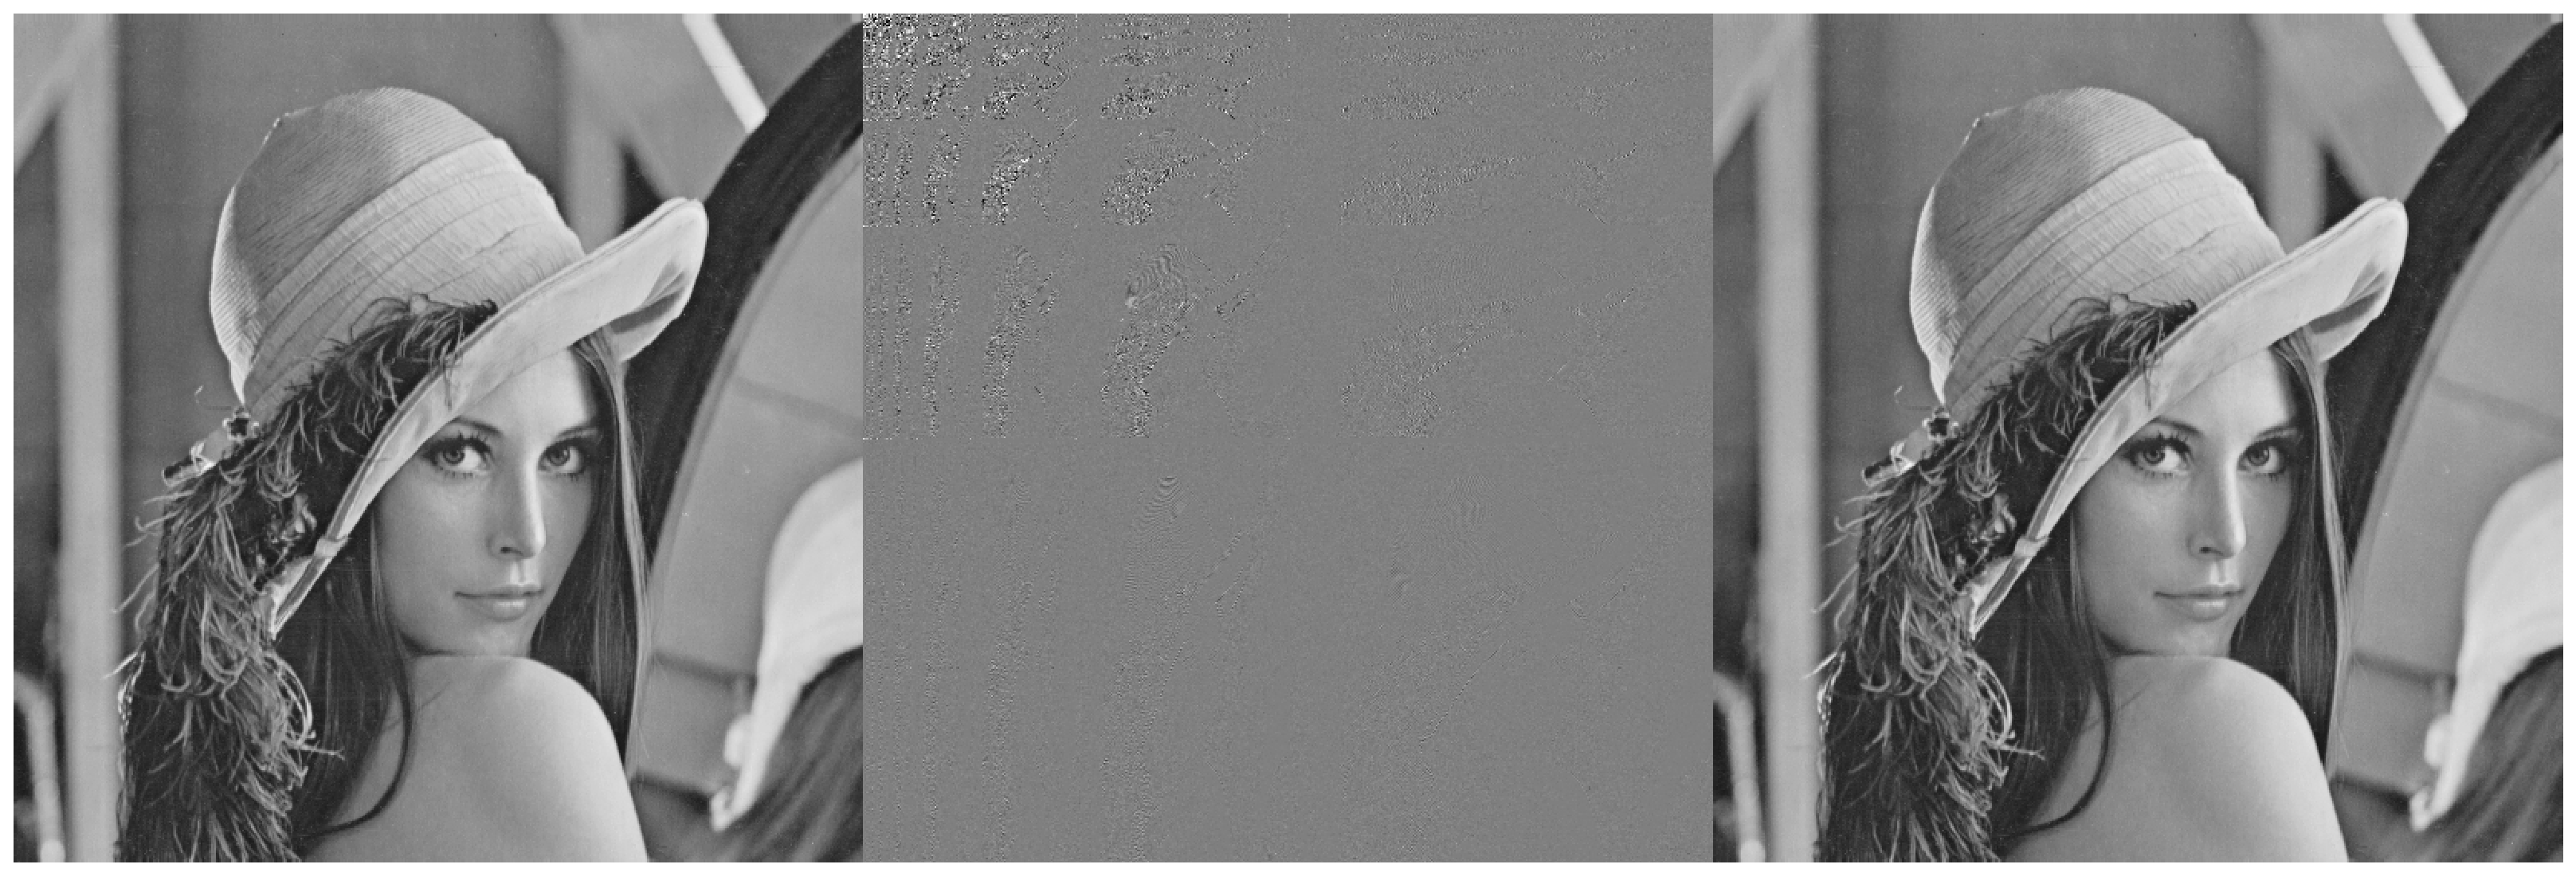
\includegraphics[width=150mm]{u05/task1.eps}
\end{center}
\caption{Original - CDF(2,2) Wavelet - R\"ucktransformation}
\end{figure}



\section*{Aufgabe 2 - Wavelet Hochpass und Gl\"attung}
\ldots
\begin{figure}[H]
\begin{center}
% 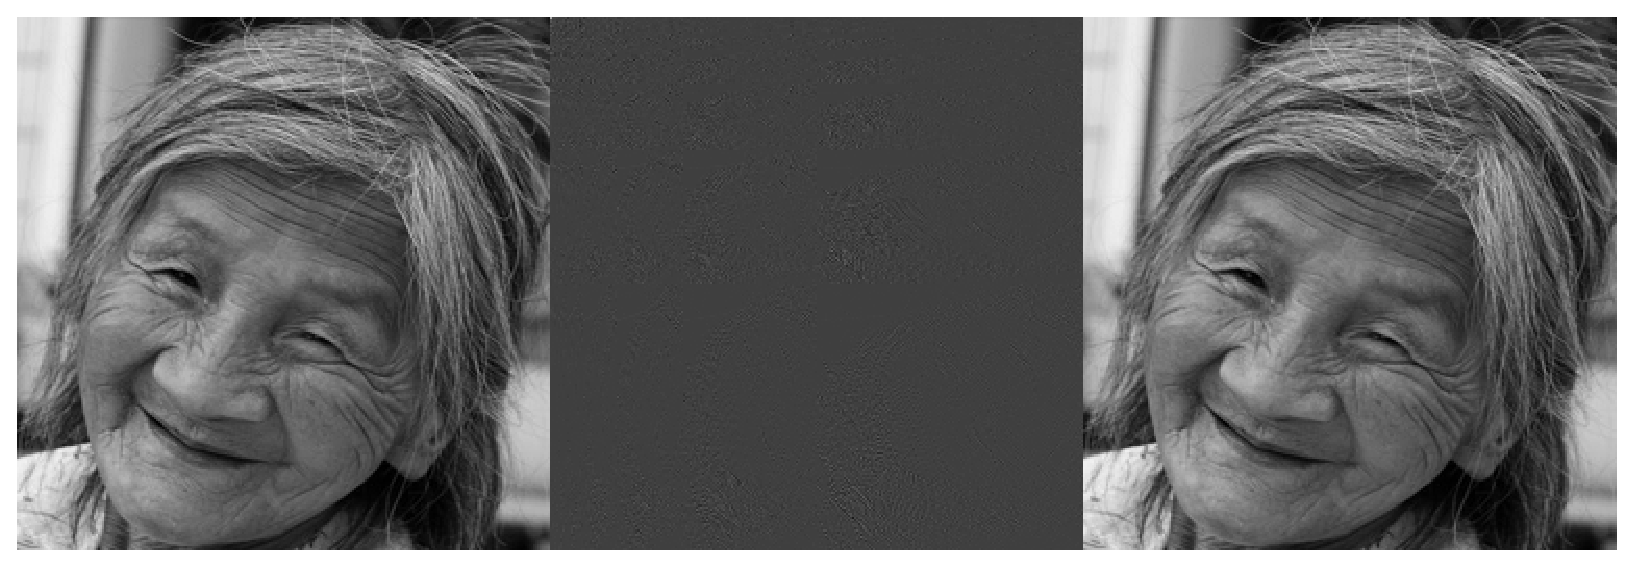
\includegraphics[width=150mm]{u05/task2.eps}
\end{center}
\caption{Wavelet Transformation}
\end{figure}


\section*{Aufgabe 3 - Lucy-Richardson Dekonvolution}
Unsere erste triviale Implementierung des Algorithmus f\"uhrte leider zu einer inakzeptablen Laufzeit, 
was uns dazu brachte die Summenberechnung per Fourier-Transformation durchzuf\"uhren. Daraus ergibt 
sich folgende vereinfachte Code-Zeile.
\begin{lstlisting}[language=matlab]
for i=1:10
    W = W.*conv(K_uni, H./conv(K_uni, W));
end
\end{lstlisting}
Der verwendete uniforme Kernel entspricht hier unserer PSF. Liest man die Zeile von hinten nach vorn,
so wird zuerst fuer alle Punkte $(x,y)$ der Einfluss von $W$ auf den Bildpunkt $H_{x,y}$ berechnet, was
der innersten Summe des Algorithmus entspricht. Danach bilden wir den Quotienten aus bekannter Bildhelligkeit und
dem soeben berechneten (rekonstruierten) original Helligkeit. Die \"aussere Summe entspricht dann der n\"achsten
Konvolution mit der PSF.
\\
Nachfolgendes Bild zeigt das Ergebnis der Dekonvolution nach 10maliger Iteration. Es ist eine Sch\"arfung zu
erkennen, doch leider nicht sehr zufrieden stellend.

\begin{figure}[H]
\begin{center}
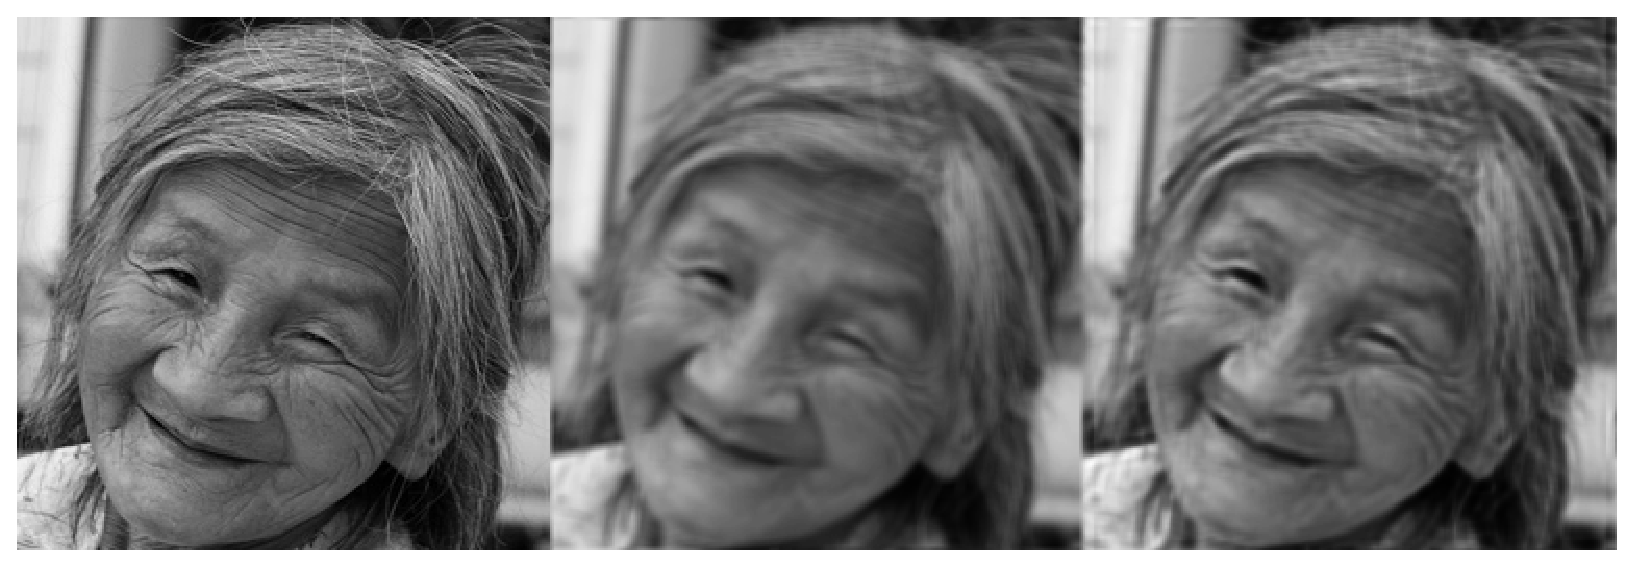
\includegraphics[width=150mm]{u05/task3.eps}
\end{center}
\caption{Original - Weichzeichnung - Nach Dekonv}
\end{figure}

\end{document}
